\documentclass[aspectratio=169,12pt]{beamer}
\usepackage[T1]{fontenc}
\usepackage{lmodern,booktabs,tikz}
\definecolor{Ink}{HTML}{17324D}
\definecolor{Teal}{HTML}{007F7B}
\definecolor{Gray}{HTML}{697887}
\definecolor{Soft}{HTML}{EEF3F6}
\setbeamercolor{normal text}{fg=Ink,bg=white}
\setbeamercolor{frametitle}{fg=Ink}
\setbeamercolor{structure}{fg=Teal}
\setbeamercolor{block title}{fg=white,bg=Teal}
\setbeamercolor{block body}{fg=Ink,bg=Soft}
\setbeamertemplate{navigation symbols}{}
\setbeamersize{text margin left=9mm,text margin right=9mm}
\setbeamerfont{frametitle}{size=\Large,series=\bfseries}
\setbeamertemplate{footline}{\hspace{9mm}\scriptsize Preliminary findings | Alex Towell\hfill\insertframenumber/5\hspace{9mm}\vspace{3mm}}
\newcommand{\aside}[1]{\vfill{\footnotesize\color{Gray}#1\par}}
\hypersetup{pdftitle={Teaching a model to find what it needs},pdfauthor={Alex Towell}}
\begin{document}

\begin{frame}[t]
\frametitle{How should a model and its tools share the work?}
Our long-term aim is to solve unfamiliar tasks by breaking them into smaller steps. A recursive language model (RLM) uses code and can ask other models for help.
\begin{block}{Before adding helpers, we test two basic questions.}
What examples teach a model to find the information it needs?\par
Which details should code handle instead of the model?
\end{block}
\textbf{Our test: a crafting game.} To make a pickaxe, the model must look up recipes, make the parts, and assemble the item.
\medskip

The game checks whether the requested item was actually made, not whether the answer sounds convincing.
\aside{Pickaxe example simplified. We use TextCraft and one small model with tools. These experiments do not yet test recursive helper calls.}
\end{frame}

\begin{frame}[t]
\frametitle{Can examples teach a model how to choose its steps?}
We train copies of the same model to imitate the next action in a worked example. This is \textbf{supervised fine-tuning (SFT)}.
\begin{block}{One simplified training example}
\textbf{Situation:} ``Make a pickaxe. Its recipe is not known yet.''\par
\textbf{Action to learn:} ``Ask the game for the pickaxe recipe.''
\end{block}
\begin{columns}[T,onlytextwidth]
\begin{column}{.48\textwidth}
\begin{block}{The teacher knows recipes.}
It uses known recipes to plan the steps, then demonstrates lookups and actions.
\end{block}
\end{column}
\begin{column}{.48\textwidth}
\begin{block}{The teacher discovers recipes.}
It looks up the goal's recipe, then its parts' recipes, to find the steps.
\end{block}
\end{column}
\end{columns}
\aside{Both teachers are programs; both demonstrate lookups on the same 32 training tasks. They differ in how the route is found, action order, and text.}
\end{frame}

\begin{frame}[t]
\frametitle{The discovery examples led to more finished tasks.}
Each model made \textbf{32 attempts}: two on each of 16 evaluation tasks. We repeated training twice. Higher bars mean more successes.
\vspace{1mm}
\begin{center}
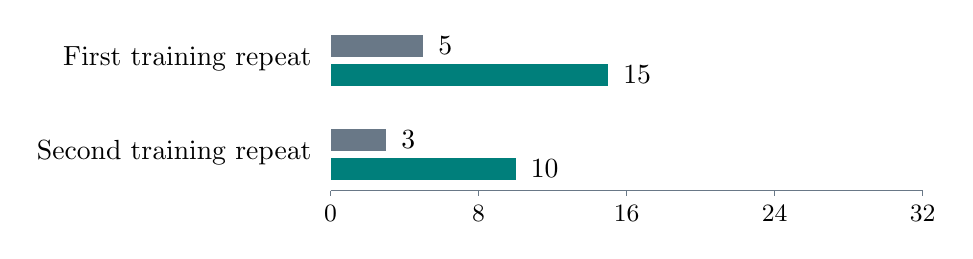
\begin{tikzpicture}[x=.235cm,y=.46cm,font=\normalsize]
\node[anchor=east] at (-.5,3.35) {First training repeat};
\node[anchor=east] at (-.5,.75) {Second training repeat};
\fill[Gray] (0,3.4) rectangle (5,4);
\fill[Teal] (0,2.6) rectangle (15,3.2);
\fill[Gray] (0,.8) rectangle (3,1.4);
\fill[Teal] (0,0) rectangle (10,.6);
\node[anchor=west] at (5.3,3.7) {5};
\node[anchor=west] at (15.3,2.9) {15};
\node[anchor=west] at (3.3,1.1) {3};
\node[anchor=west] at (10.3,.3) {10};
\draw[Gray] (0,-.3)--(32,-.3);
\foreach \n in {0,8,16,24,32} {\draw[Gray] (\n,-.3)--(\n,-.45);\node[below,font=\small] at (\n,-.45) {\n};}
\end{tikzpicture}
\end{center}
{\small\color{Gray}\rule{4mm}{2mm} Teacher knows recipes\quad\color{Teal}\rule{4mm}{2mm} Teacher discovers recipes}
\medskip

With changed recipes, discovery also led: \textbf{6 vs.\ 4} and \textbf{8 vs.\ 1} successes out of 16. The smaller lead is uncertain.
\aside{The first teacher's quantity error is corrected. These tests helped us develop the approach; a separate final test is still needed.}
\end{frame}

\begin{frame}[t]
\frametitle{Code can handle details without choosing the plan.}
A model can read the right recipe but still send the wrong ingredients. We changed the tool, with \textbf{no extra training}:
\medskip

\textbf{The model chooses} what to make and how much.\par
\textbf{Code fills in} ingredients from a recipe already looked up.
\vspace{1mm}
\begin{center}
\renewcommand{\arraystretch}{1.05}
\begin{tabular}{lcc}
\toprule
Successful attempts & Model fills & Code fills\\
(out of 16) & ingredients & ingredients\\
\midrule
Recipe set A, first trained model & 6 & \textbf{12}\\
Recipe set A, second trained model & 8 & \textbf{10}\\
Recipe set B, first trained model & 9 & \textbf{14}\\
Recipe set B, second trained model & 9 & \textbf{13}\\
\bottomrule
\end{tabular}
\end{center}
\aside{A and B change the recipes and supplies for the same eight goals. Both models learned from discovery. The smallest gain is uncertain; all outcomes are known.}
\end{frame}

\begin{frame}[t]
\frametitle{The promising direction is learning and tools together.}
\begin{block}{What we learned in these small tests}
Examples that discover the steps worked better than examples from a teacher that already knew them.\par
\medskip
Letting code handle recipe details helped without changing the model's training.
\end{block}
\textbf{What we have not shown:} that this works beyond crafting, or that adding recursive helpers improves planning.
\medskip

\textbf{Next test:} On new goals, does code help both kinds of trained model? Does the discovery advantage remain?
\medskip

\textbf{For discussion:} What other multi-step task would make this a convincing result?
\aside{The broader comparison is queued. It is future evidence, not a result claimed here.}
\end{frame}
\end{document}
